\documentclass{article}
\usepackage{graphicx, ctex, float}
\begin{document}
  \section{ValueNet简介}  
  \subsection{功能}
    对一段给定的音符序列打分,衡量其是“我们所倾向的音乐”的程度。
  \subsection{目的}
    设计这个神经网络的最初目的
    是用来代替作曲网络(CompoNet)原来的cost函数,使训练目标更接近于“是音乐”而不是
    “和训练用的音乐一致”,但后来发现受到技术的限制,我们无法完成这种替换,于是又想到可以
    把它作为遗传算法的适应度计算函数。
  \subsection{输入}
    为了避免音符四个要素的数值大小差别太大造成的问题,基于统计出的四个要素的数值分布,
    我们设计了四个压缩函数来将四个要素的数值分别映射到0到1之间。
    \subsubsection{压缩pitch与dynamic}
      对于pitch和dynamic的压缩基于sigmoid函数,因为这两者的分布比较集中于某个
      中间值,而sigmoid函数在中间部分很陡峭,适合将“密集”的值分散开。
      压缩函数为:
      \[f_{pitch}(x) = \frac{1}{1+e^\frac{x-58}{12}}\]
      \[f_{dynamic}(x) = \frac{1}{1+e^\frac{x-75}{16}}\]
      其中的具体参数是通过估算和实验确定的。
      压缩前后的分布对比如图\ref{statistics1}:
      \begin{figure}[H]
      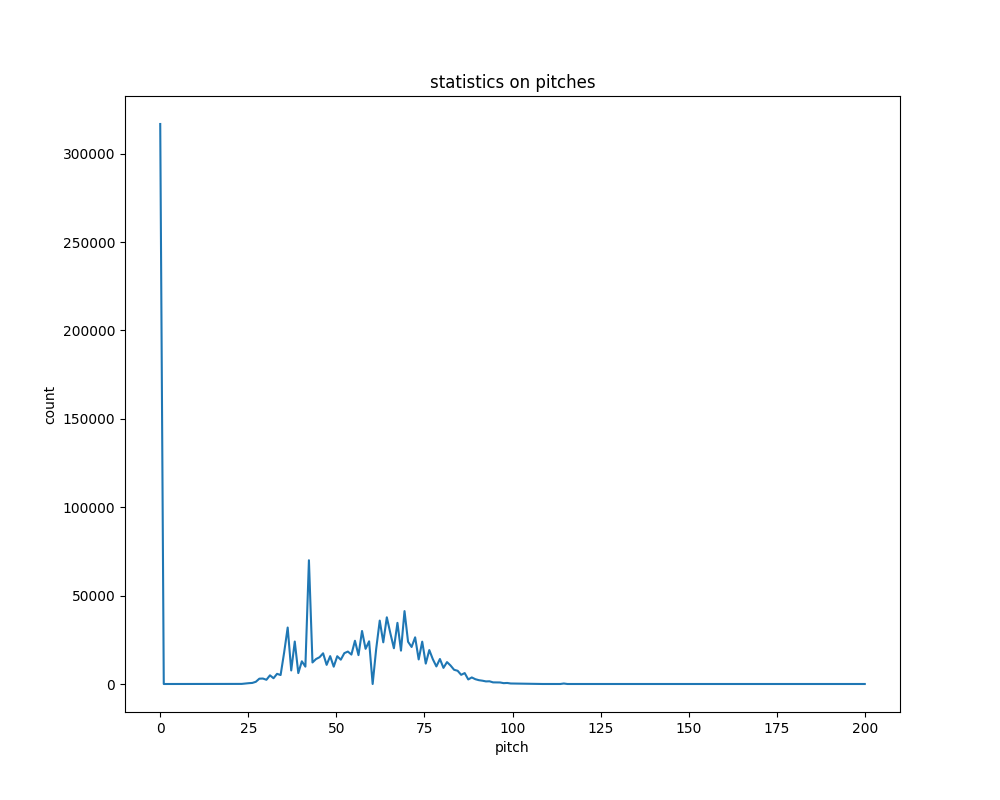
\includegraphics[width=.45\textwidth]{picture/pitches.png}
      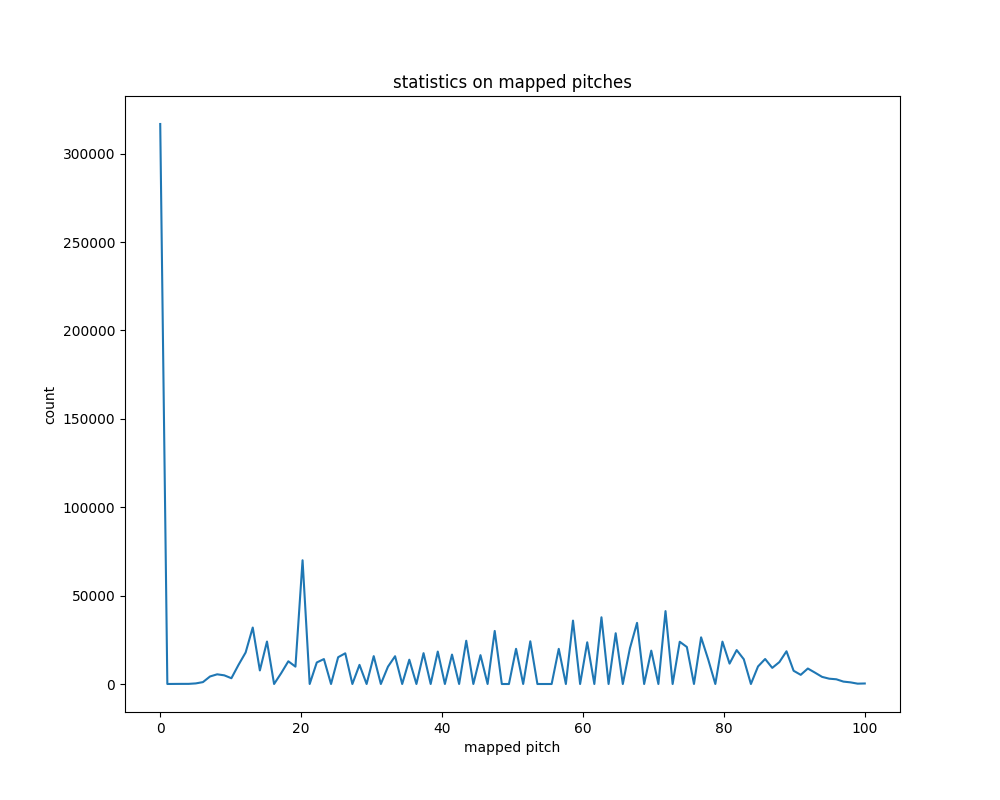
\includegraphics[width=.45\textwidth]{picture/pitches_mapped.png}

      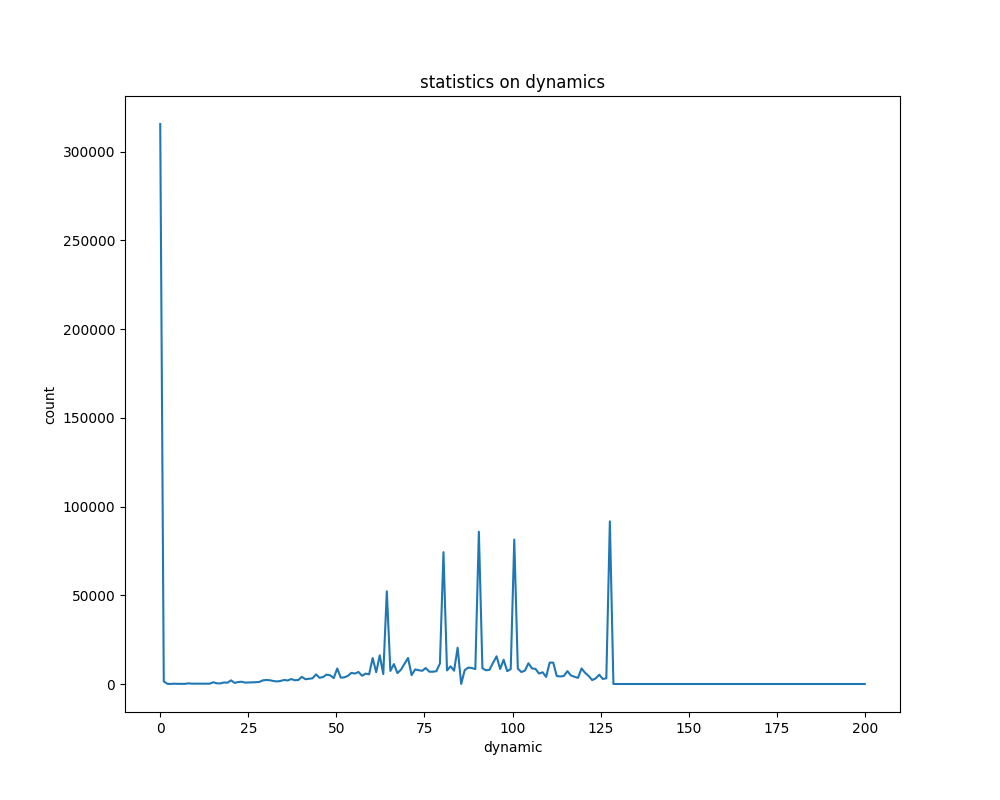
\includegraphics[width=.45\textwidth]{picture/dynamics.png}
      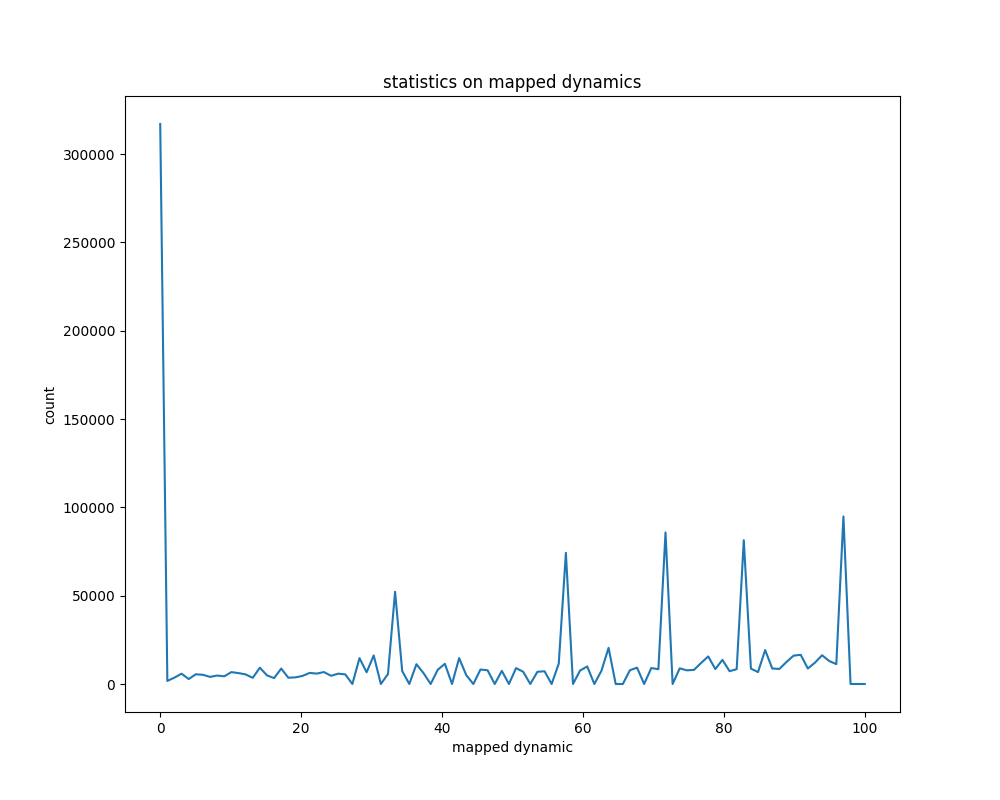
\includegraphics[width=.45\textwidth]{picture/dynamics_mapped.png}
      \caption{pitch、dynamic压缩前后分布}
      \label{statistics1}
      \end{figure}
    \subsubsection{压缩rhythmValue与duration}
      对于rhythmValue和duration的压缩基于对数函数,因为它们的原始取值的分布呈先密集后
      稀疏的特点,而对数函数先陡峭后平缓,有助于使压缩后的分布趋于均匀。
      压缩函数为:
      \[f_{rhythmValue}(x) = \log_{800}{200x}\]
      \[f_{duration}(x) = \log_{500}{50x}\]
      压缩前后的分布如图\ref{statistics2}:
      \begin{figure}[H]
      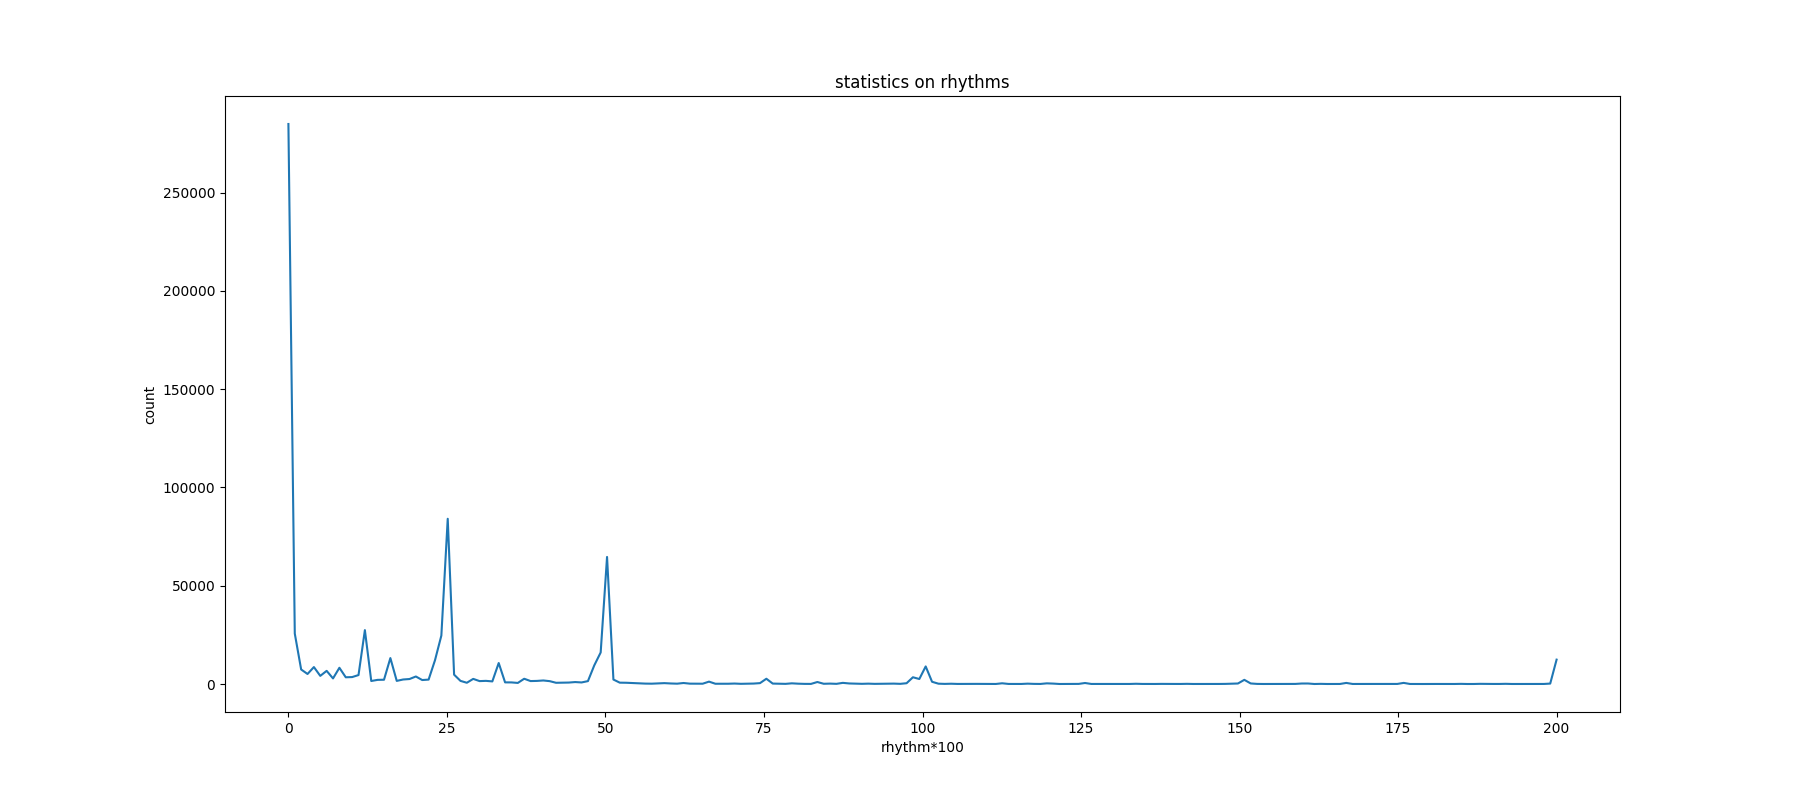
\includegraphics[width=.45\textwidth]{picture/rhythms.png}
      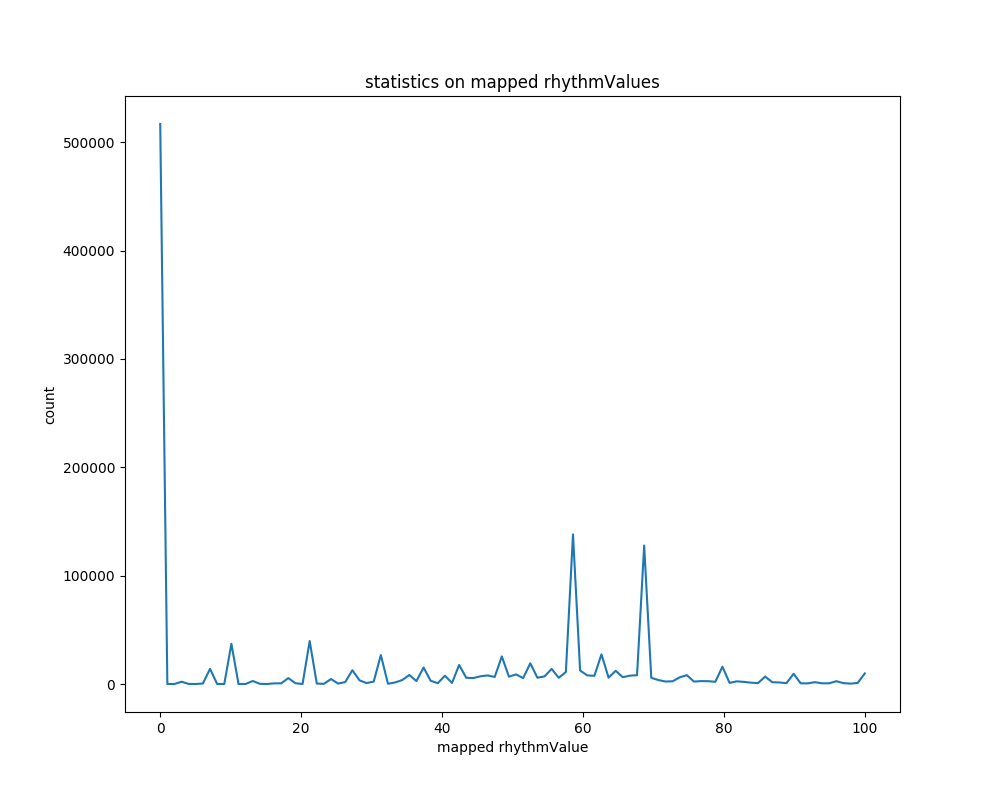
\includegraphics[width=.45\textwidth]{picture/rhythms_mapped.png}
      
      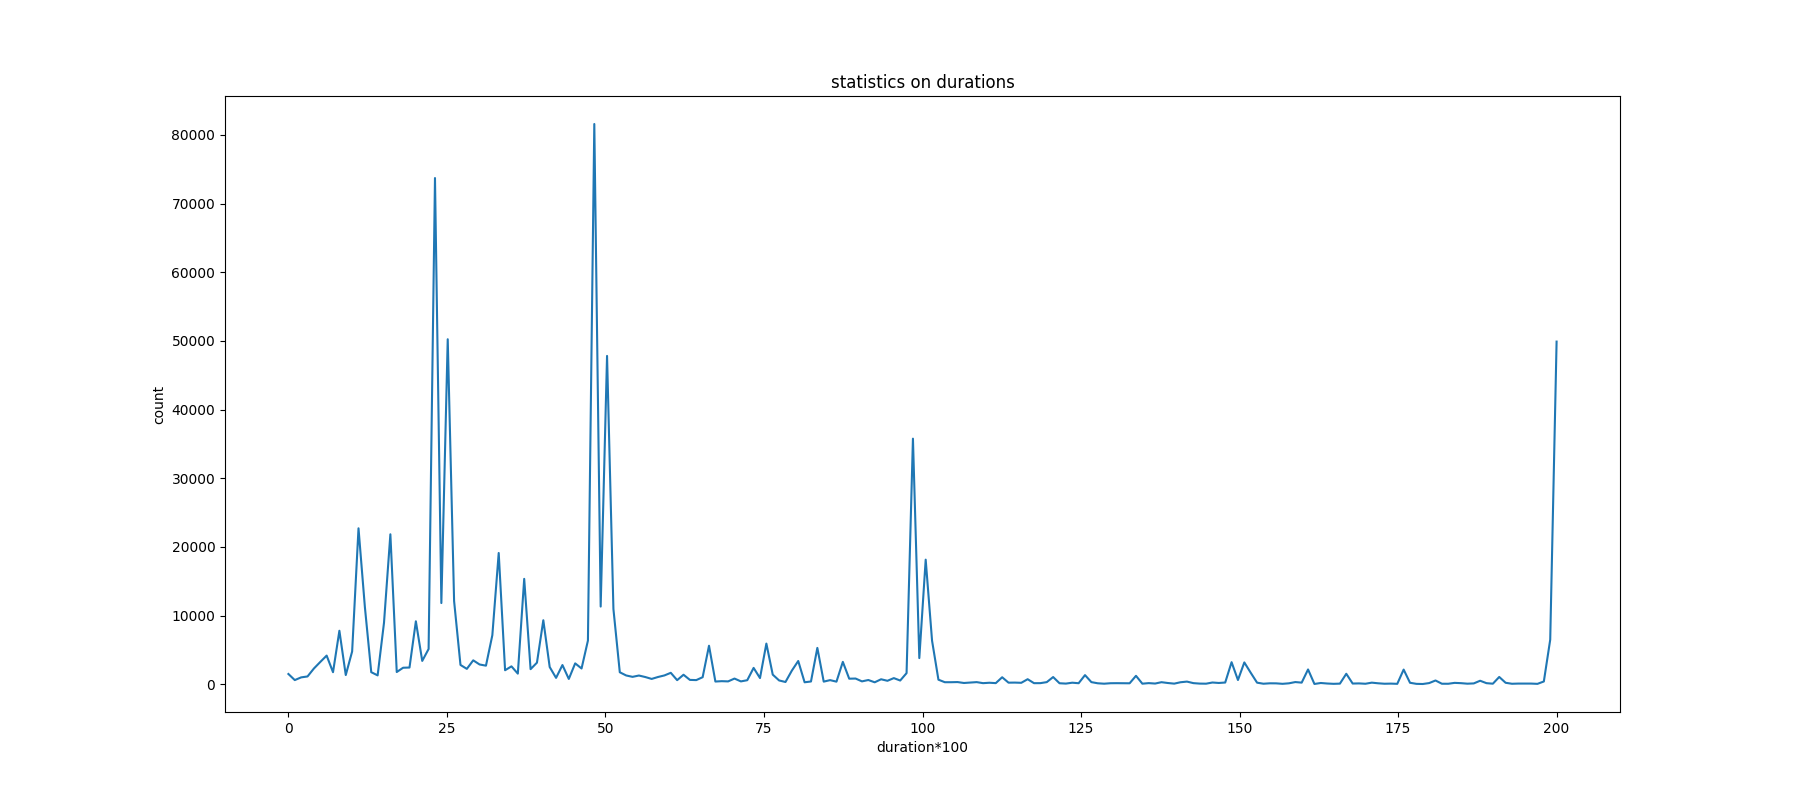
\includegraphics[width=.45\textwidth]{picture/durations.png}
      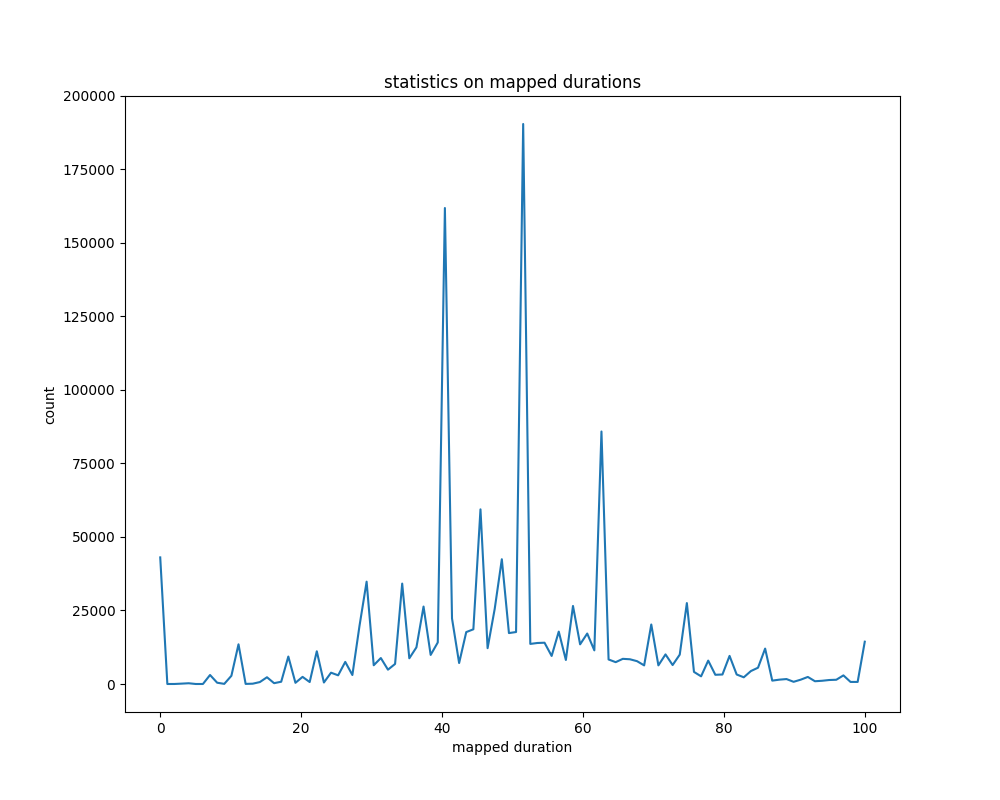
\includegraphics[width=.45\textwidth]{picture/durations_mapped.png}
      \caption{rhythmValue、duration压缩前后分布}
      \label{statistics2}      
      \end{figure}
  \subsection{结构和训练}
    我们使用了卷积神经网络(CNN)而不是擅长处理序列的递归神经网络(RNN),原因是我们
    认为音乐具有相当强
    的局部特征,利用CNN的卷积层和池化层可以提取其局部特征,而提取后的
    局部特征在全连接层被处理又有一种“考虑全曲的情感变化”的感觉,因此我们觉得这很适合用
    CNN来处理。
    输入是一维的,有四个channel(即音符的四个要素)。
    第一层为卷积层,感受野宽度为8,卷积核数为8。
    第二层为池化层,池化方式为平均池化,池化宽度为4。
    第三层为卷积层,感受野宽度为4,卷积核数为16。
    第四层为池化层,池化方式为平均池化,池化宽度为8。
    第五层为全连接层,输出为一个数值,我们将它视作该网络对输入序列的评分。

    我们手工对一些曲子进行了打分,分为1.0、0.6、0.4、0.0,1.0主要是莫扎特的作品,
    0.6和0.4是凭感觉在已有的midi文件中选出来的,0.0是随机生成的。
  \subsection{效果}
    在训练了足够长的时间后,我们在训练数据上进行了评分效果的评估,将网络的输出
    与给出的标签差距小于0.1的视为正确,正确率如下:
      % TODO
    经过抽样对比神经网络评分与标签的差别,我们发现虽然有时误差大于0.1,
    但神经网络给出的评分还是和标签很接近的。
\end{document}
